% !TEX root = ../main.tex
\chapter{Breadboard Prototyping \& Circuit Troubleshooting}

\section{Internal Architecture of Solderless Breadboards}
A solderless breadboard is an essential modular platform for rapid temporary circuit prototyping \cite{sparkfun_breadboard}. The internal architecture consists of molded thermoplastic housing enclosing spring-tempered phosphor bronze or nickel-silver clip strips:

\begin{enumerate}[leftmargin=1.5em]
    \item \textbf{Distribution Buses (Power Rails):} Longitudinal outer strips marked with red ($+$) and blue/black ($-$) color lines. These rails distribute DC supply voltage ($V_{CC}$) and system ground (GND) across the entire prototyping area.
    \item \textbf{Terminal Strips (Component Rows):} Arranged in vertical 5-hole tie-point groups. All 5 socket holes in a given column group are electrically bonded together by a common spring clip beneath the surface.
    \item \textbf{Central DIP Isolation Channel:} A $0.3\text{-inch}$ ($7.62\text{ mm}$) groove dividing the board halves. This channel matches standard Dual In-Line Package (DIP) IC lead spacing, ensuring opposing pins remain electrically isolated.
\end{enumerate}

\begin{figure}[htbp]
    \centering
    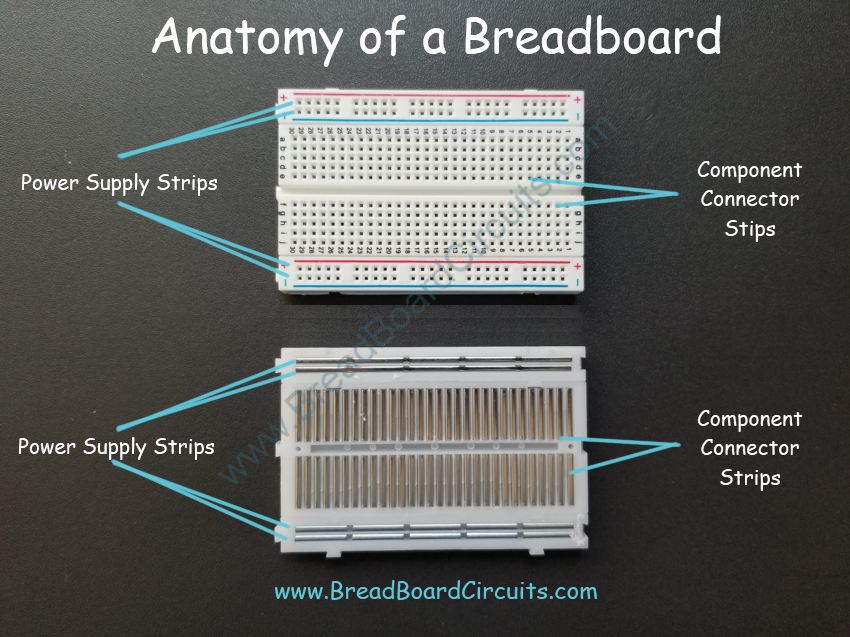
\includegraphics[width=0.78\textwidth]{figures/fig_breadboard_internal.jpg}
    \caption{Anatomy of a solderless breadboard showing the top face alongside the exposed reverse side, revealing the underlying metallic power distribution buses and vertical component terminal clip rows \cite{breadboardcircuits_anatomy}.}
    \label{fig:breadboard_internal}
\end{figure}

\section{Systematic Circuit Troubleshooting Methodology}
When an assembled prototype circuit fails to operate, technicians must avoid random component swapping. Systematic diagnostic methodology isolates the root cause rapidly:

\subsection{Step 1: Visual and Tactile Inspection (Power OFF)}
With power completely de-energized:
\begin{itemize}[leftmargin=1.5em]
    \item Verify semiconductor polarity: check LED anode/cathode orientation, electrolytic capacitor polarity bands, and diode cathode stripe bands.
    \item Inspect IC alignment: ensure the index notch/dot faces Pin 1 and no pins are folded or bent under the IC package.
    \item Check jumper seating: confirm wires are firmly seated in active terminal rows rather than loose or bridged across adjacent rows.
\end{itemize}

\subsection{Step 2: Static Power Supply Verification (Power ON)}
Energize the DC power supply:
\begin{itemize}[leftmargin=1.5em]
    \item Measure DC voltage directly at the breadboard power rail tie-points using a Digital Multimeter (DMM).
    \item Verify that rail voltage matches expected supply levels without excessive voltage drooping caused by power supply current limits or rail shorts.
\end{itemize}

\subsection{Step 3: Point-to-Point Node Voltage Tracing}
With circuit power active:
\begin{itemize}[leftmargin=1.5em]
    \item Secure the black DMM probe to system ground (GND).
    \item Progressively probe circuit nodes with the red DMM probe along the schematic signal path from source to load.
    \item Compare each measured DC node voltage against theoretical schematic calculations. A sudden divergence reveals open circuits, floating inputs, or defective components.
\end{itemize}

\subsection{Step 4: Resistance and Continuity Isolation (Power OFF)}
De-energize circuit power:
\begin{itemize}[leftmargin=1.5em]
    \item Set the DMM to audible continuity/resistance mode.
    \item Probe between nodes to verify low-resistance ($<1\ \Omega$) paths along expected traces and high-impedance ($>1\text{ M}\Omega$) isolation between adjacent, independent breadboard rows.
\end{itemize}
